%%%%%%%%%%%%%%%%%%%%%%%%%%%%%%%%%%%%%%%%%
% Beamer Presentation
% LaTeX Template
% Version 1.0 (10/11/12)
%
% This template has been downloaded from:
% http://www.LaTeXTemplates.com
%
% License:
% CC BY-NC-SA 3.0 (http://creativecommons.org/licenses/by-nc-sa/3.0/)
%
%%%%%%%%%%%%%%%%%%%%%%%%%%%%%%%%%%%%%%%%%

%----------------------------------------------------------------------------------------
%	PACKAGES AND THEMES
%----------------------------------------------------------------------------------------

\documentclass[handout]{beamer}

\mode<presentation> {

% The Beamer class comes with a number of default slide themes
% which change the colors and layouts of slides. Below this is a list
% of all the themes, uncomment each in turn to see what they look like.

%\usetheme{default}
%\usetheme{AnnArbor}
%\usetheme{Antibes}
%\usetheme{Bergen}
%\usetheme{Berkeley}
%\usetheme{Berlin}
%\usetheme{Boadilla}
%\usetheme{CambridgeUS}
%\usetheme{Copenhagen}
%\usetheme{Darmstadt}
%\usetheme{Dresden}
%\usetheme{Frankfurt}
%\usetheme{Goettingen}
%\usetheme{Hannover}
%\usetheme{Ilmenau}
%\usetheme{JuanLesPins}
%\usetheme{Luebeck}
\usetheme{Madrid}
%\usetheme{Malmoe}
%\usetheme{Marburg}
%\usetheme{Montpellier}
%\usetheme{PaloAlto}
%\usetheme{Pittsburgh}
%\usetheme{Rochester}
%\usetheme{Singapore}
%\usetheme{Szeged}
%\usetheme{Warsaw}

% As well as themes, the Beamer class has a number of color themes
% for any slide theme. Uncomment each of these in turn to see how it
% changes the colors of your current slide theme.

%\usecolortheme{albatross}
%\usecolortheme{beaver}
%\usecolortheme{beetle}
%\usecolortheme{crane}
%\usecolortheme{dolphin}
%\usecolortheme{dove}
%\usecolortheme{fly}
%\usecolortheme{lily}
%\usecolortheme{orchid}
%\usecolortheme{rose}
%\usecolortheme{seagull}
%\usecolortheme{seahorse}
%\usecolortheme{whale}
%\usecolortheme{wolverine}

%\setbeamertemplate{footline} % To remove the footer line in all slides uncomment this line
%\setbeamertemplate{footline}[page number] % To replace the footer line in all slides with a simple slide count uncomment this line

%\setbeamertemplate{navigation symbols}{} % To remove the navigation symbols from the bottom of all slides uncomment this line
}

\usepackage{graphicx} % Allows including images
\usepackage{booktabs} % Allows the use of \toprule, \midrule and \bottomrule in tables
\usepackage{cool}
\usepackage{tikz}
\usepackage{amsmath}
\usepackage{MnSymbol,wasysym}
\DeclareMathOperator*{\argmax}{argmax}
\DeclareMathOperator*{\argmin}{argmin}
\usetikzlibrary{positioning}

%----------------------------------------------------------------------------------------
%	TITLE PAGE
%----------------------------------------------------------------------------------------

\title[A.I. For Retail]{A.I. for Optimal Decisioning under Uncertainty} % The short title appears at the bottom of every slide, the full title is only on the title page
\subtitle{Applied to Inventory and Price Optimization}
\author{Ashwin Rao} % Your name
\institute[Target/Stanford] % Your institution as it will appear on the bottom of every slide, may be shorthand to save space
{V.P. Artificial Intelligence at Target \& Adjunct Faculty at Stanford
 % Your institution for the title page
}
\date{\today} % Date, can be changed to a custom date

\begin{document}
\begin{frame}
\titlepage % Print the title page as the first slide
\end{frame}

\begin{frame}
\frametitle{Meet the Speaker}
\pause
\begin{itemize}[<+->]
\item Here at Target, V.P. of Artificial Intelligence team in Data Sciences
\item Other Job: Adjunct Faculty in Applied Math at Stanford University
\item Director of Stanford's Mathematical \& Comp. Finance program
\item At Stanford, I teach a course on \href{https://github.com/coverdrive/technical-documents/blob/master/finance/cme241/Stanford-CME241.pdf}{\underline{\textcolor{blue}{Reinforcement Learning for Finance}}}
\item I've written an \href{https://github.com/coverdrive/MDP-DP-RL}{\underline{\textcolor{blue}{educational codebase}}} for Reinforcement Learning
\item Previously, 14 years in Derivatives Trading at GS and MS in NY
\item My teaching has been in Pure \& Applied Math, Comp Sci, Finance
\item My original background is Algorithms Theory \& Abstract Algebra
\end{itemize}
\end{frame}

\begin{frame}
\frametitle{Overview} % Table of contents slide, comment this block out to remove it
\tableofcontents % Throughout your presentation, if you choose to use \section{} and \subsection{} commands, these will automatically be printed on this slide as an overview of your presentation
\end{frame}

\section{The Framework of Stochastic Control}

\begin{frame}
\frametitle{A.I. for Optimal/Dynamic Decisioning under Uncertainty}
\pause
\begin{itemize}[<+->]
\item Let's look at some terms we use to characterize this branch of A.I.
\item {\em Stochastic}: Uncertainty in key quantities, evolving over time
\item {\em Optimization}: A well-defined metric to be maximized (``The Goal'')
\item {\em Dynamic}:  Decisions need to a function of the changing situations
\item {\em Control}: Overpower uncertainty by persistent steering towards goal
\item Jargon overload due to confluence of Control Theory, O.R. and A.I.
\item For language clarity, let's just refer to this area as {\em Stochastic Control}
\item The core framework is called {\em Markov Decision Processes} (MDP)
\item {\em Reinforcement Learning} is a class of algorithms to solve MDPs
\end{itemize}
\end{frame}


\begin{frame}
\frametitle{The MDP Framework}
\includegraphics[width=12cm, height=7cm]{../finance/cme241/MDP.png}
\end{frame}

\begin{frame}
\frametitle{Components of the MDP Framework}
\pause
\begin{itemize}[<+->]
\item The {\em Agent} and the {\em Environment} interact in a time-sequenced loop
\item {\em Agent} responds to [{\em State}, {\em Reward}] by taking an {\em Action}
\item {\em Environment} responds by producing next step's (random) {\em State}
\item {\em Environment} also produces a (random) scalar denoted as {\em Reward}
\item Each {\em State} is assumed to have the {\em Markov Property}, meaning:
\begin{itemize}
\item Next {\em State/Reward} depends only on Current {\em State} (for a given {\em Action})
\item Current {\em State} captures all relevant information from {\em History}
\item Current {\em State} is a sufficient statistic of the future (for a given {\em Action})
\end{itemize} 
\item Goal of {\em Agent} is to maximize {\em Expected Sum} of all future {\em Reward}s
\item By controlling the ({\em Policy} : {\em State} $\rightarrow$ {\em Action}) function
\item This is a dynamic (time-sequenced control) system under uncertainty
\end{itemize}
\end{frame}

\begin{frame}
\frametitle{Formal MDP Framework}
The following notation is for discrete time steps. Continuous-time formulation is analogous (often involving
\href{https://github.com/coverdrive/technical-documents/blob/master/finance/cme241/StochasticCalculusFoundations.pdf}{\underline{\textcolor{blue}{Stochastic Calculus}}})
\pause
\begin{itemize}[<+->]
\item Time steps denoted as $t = 1, 2, 3, \ldots$
\item Markov States $S_t \in \mathcal{S}$ where $\mathcal{S}$ is the State Space
\item Actions $A_t \in \mathcal{A}$ where $\mathcal{A}$ is the Action Space
\item Rewards $R_t \in \mathbb{R}$ denoting numerical feedback\
\item Transitions $p(s',r|s,a) = Pr\{S_{t+1}=s',R_{t+1}=r|S_t=s,A_t=a\}$
\item $\gamma \in [0,1]$ is the Discount Factor for Reward when defining {\em Return}
\item Return $G_t = R_{t+1} + \gamma \cdot R_{t+2} + \gamma^2 \cdot R_{t+3} + \ldots$
\item Policy $\pi(a|s)$ is probability that Agent takes action $a$ in states $s$
\item The goal is find a policy that maximizes  $\mathbb{E}[G_t|S_t = s]$ for all $s \in \mathcal{S}$
\end{itemize}
\end{frame}

\begin{frame}
\frametitle{How a baby learns to walk}
\includegraphics[width=13cm, height=8cm]{../finance/cme241/BabyMDP.jpg}
\end{frame}

\begin{frame}
\frametitle{Many real-world problems fit this MDP framework}
\pause
\begin{itemize}[<+->]
\item Self-driving vehicle (speed/steering to optimize safety/time)
\item Game of Chess (Boolean {\em Reward} at end of game)
\item Complex Logistical Operations (eg: movements in a Warehouse)
\item Make a humanoid robot walk/run on difficult terrains
\item Manage an investment portfolio
\item Control a power station
\item Optimal decisions during a football game
\item Strategy to win an election (high-complexity MDP)
\end{itemize}
\end{frame}

\begin{frame}
\frametitle{Self-Driving Vehicle}
\includegraphics[width=13cm, height=8cm]{../finance/cme241/CarMDP.jpg}
\end{frame}

\begin{frame}
\frametitle{Why are these problems hard?}
\pause
\begin{itemize}[<+->]
\item {\em State} space can be large or complex (involving many variables)
\item Sometimes, {\em Action} space is also large or complex
\item No direct feedback on ``correct'' {\em Actions} (only feedback is {\em Reward})
\item Time-sequenced complexity ({\em Actions} influence future {\em States/Actions})
\item {\em Action}s can have delayed consequences (late {\em Reward}s)
\item {\em Agent} often doesn't know the {\em Model} of the {\em Environment}
\item ``Model'' refers to probabilities of state-transitions and rewards
\item So, {\em Agent} has to learn the {\em Model} AND solve for the Optimal {\em Policy}
\item {\em Agent} {\em Action}s need to tradeoff between ``explore'' and ``exploit''
\end{itemize}
\end{frame}

\begin{frame}
\frametitle{Value Function and Bellman Equations}
\pause
\begin{itemize}
\item Value function (under policy $\pi$) $V_{\pi}(s) = \mathbb{E}[G_t|S_t = s]$ for all $s \in \mathcal{S}$
\pause
$$V_{\pi}(s) = \sum_{a} \pi(a|s) \sum_{s',r} p(s',r|s,a) \cdot (r + \gamma V_{\pi}(s')) \mbox{ for all } s \in \mathcal{S}$$
\pause
\item Optimal Value Function $V_{*}(s) = \max_{\pi} V_{\pi}(s) \mbox{ for all } s \in \mathcal{S}$
\pause
$$V_{*}(s) = \max_{a} \sum_{s',r} p(s',r|s,a) \cdot (r + \gamma V_{*}(s')) \mbox{ for all } s \in \mathcal{S}$$
\pause
\item {\em There exists an Optimal Policy} $\pi_{*}$ achieving $V_{*}(s)$ for all $s \in \mathcal{S}$
\pause
\item Determining $V_{\pi}(s)$ known as {\em Prediction}, and $V_{*}(s)$ known as {\em Control}
\pause
\item The above recursive equations are called {\em Bellman equations}
\pause
\item In continuous time, refered to as {\em Hamilton-Jacobi-Bellman (HJB)}
\pause
\item The algorithms based on Bellman equations are broadly classified as:
\begin{itemize}
\item Dynamic Programming
\item Reinforcement Learning
\end{itemize}

\end{itemize}
\end{frame}


\begin{frame}
\frametitle{Dynamic Programming versus Reinforcement Learning}
\pause
\begin{itemize}[<+->]
\item When Probabilities Model is known $\Rightarrow$ {\em Dynamic Programming} (DP)
\item DP Algorithms take advantage of knowledge of probabilities
\item So, DP Algorithms do not require interaction with the environment
\item In the Language of A.I, DP is a type of {\em Planning Algorithm}
\item When Probabilities Model unknown $\Rightarrow$ {\em Reinforcement Learning} (RL)
\item RL Algorithms interact with the Environment and incrementally learn
\item Environment interaction could be {\em real} or {\em simulated} interaction
\item RL approach: Try different actions \& learn what works, what doesn't
\item RL Algorithms' key challenge is to tradeoff ``explore'' versus ``exploit''
\item DP or RL, Good approximation of Value Function is vital to success
\item Deep Neural Networks are typically used for function approximation
\end{itemize}
\end{frame}


\begin{frame}
\frametitle{Why is RL interesting/useful to learn about?}
\pause
\begin{itemize}[<+->]
\item RL solves MDP problem when {\em Environment Probabilities} are unknown
\item This is typical in real-world problems (complex/unknown probabilities)
\item RL interacts with {\em Actual Environment} or with {\em Simulated Environment}

\item {\bf Promise of modern A.I. is based on success of RL algorithms}
\item Potential for automated decision-making in many industries
\item In 10-20 years: Bots that act or behave more optimal than humans
\item RL already solves various low-complexity real-world problems
\item RL might soon be the most-desired skill in the technical job-market
\item Learning RL is a lot of fun! (interesting in theory as well as coding)
\end{itemize}
\end{frame}

\begin{frame}
\frametitle{Many Faces of Reinforcement Learning}
\includegraphics[width=9cm, height=8cm]{../finance/cme241/many_faces_of_RL.PNG}
\end{frame}

\begin{frame}
\frametitle{Vague (but in-vogue) Classification of Machine Learning}
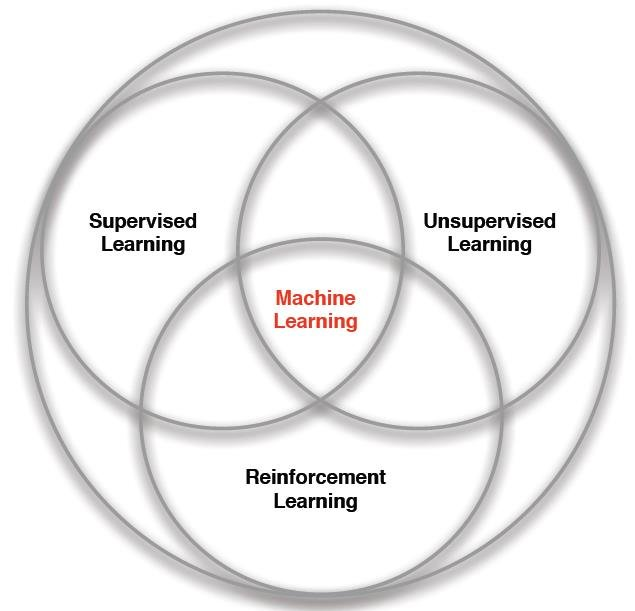
\includegraphics[width=9cm, height=8cm]{../finance/cme241/MLBranches.PNG}
\end{frame}


\section{Inventory Optimization}

\begin{frame}
\frametitle{Inventory Optimization}
\pause
\begin{itemize}[<+->]
\item A fundamental problem in Retail is Inventory Optimization
\item How to move inventory optimally from vendors to guests
\item Guest Demand is fairly uncertain
\item Nirvana is when Inventory appears ``just in time'' to satisfy Demand
\item This is an example of a Stochastic Control problem
\end{itemize}
\end{frame}


\begin{frame}
\frametitle{Single-store, Single-item Inventory Optimization}
\pause
\begin{itemize}[<+->]
\item The store experiences random daily demand given by PDF $f(x)$
\item The store can order daily from a vendor carrying infinite inventory
\item There's a cost associated with ordering, and order arrives in $L$ days
\item Holding Cost $h$ for each unit of overnight inventory
\item Stockout Cost $p$ for each unit of lost sales due to empty shelf
\item This is an MDP where {\em State} is current Inventory Position
\item {\em Action} is quantity to Order
\item {\em Reward} function has $h$, $p$, and ordering cost
\item Transition probabilities are governed by demand distribution $f(x)$
\item The Optimal (Ordering) Policy has a simple closed-form solution
\end{itemize}
\end{frame}

\begin{frame}
\frametitle{Optimal Ordering Policy}
\includegraphics[width=12cm, height=8cm]{op_otl.png}
\end{frame}


\begin{frame}
\frametitle{The Core of this Solution has this Pictorial Intuition}
\includegraphics[width=12cm, height=8cm]{newsvendor_arrow1.png}
\end{frame}


\begin{frame}
\frametitle{Costs viewed against End-of-Day Inventory}
\includegraphics[width=12cm, height=8cm]{newsvendor_arrow2.png}
\end{frame}

\begin{frame}
\frametitle{UnderCapacity and OverCapacity Costs}
\includegraphics[width=12cm, height=8cm]{capacity_costs.png}
\end{frame}

\begin{frame}
\frametitle{UnderCapacity Cost: Guest Psychology and Economics}
\pause
\begin{itemize}[<+->]
\item Retail Mantra: ``Stack it high and watch it fly''
\item Guests like to see shelves well stocked
\item Visual emptiness is known to be a sales deterrent
\item So, full-looking shelves are part of presentation strategy
\item At a certain level of emptiness, the deterrent rises sharply
\item Hence the convex nature of this cost curve
\item Note that this curve varies from item to item
\item It also varies from regular season to end of season
\item Modeling/calibrating this is tricky!
\item However, getting a basic model in place is vital
\end{itemize}
\end{frame}

\begin{frame}
\frametitle{OverCapacity Cost: Backroom Space Constraints}
\pause
\begin{itemize}[<+->]
\item Retail store backrooms have limited capacity
\item Typically tens of thousands of items compete for this space
\item Retailers like to have clean and organized backrooms
\item A perfect model is when all your inventory is on store shelves
\item With backroom used purely as a hub for home deliveries
\item Practically, some overflow from shelves is unavoidable
\item Hence, the convex nature of this curve
\item Modeling this is hard because it's a multi-item cost/constraint
\item Again, getting a basic model in place is vital
\end{itemize}
\end{frame}

\begin{frame}
\frametitle{What other costs are involved?}
\pause
\begin{itemize}[<+->]
\item Holding Cost: Interest on Inventory, Superficial Damage, Maintenance
\item Stockout Cost: Lost Sales, sometimes Lost Customers
\item Labor Cost: Replenishment involves movement from truck to shelf
\item Spoilage Cost: Food \& Beverages can have acute perishability
\item End-of-Season/Obsolescence Cost: Intersects with Clearance Pricing 
\end{itemize}
\end{frame}

\begin{frame}
\frametitle{Practical Inventory Optimization as an MDP}
\pause
\begin{itemize}[<+->]
\item The store experiences random daily demand
\item The store can place a replenishment order in casepack mutiples
\item This is an MDP where {\em State} is current Inventory Position
\item {\em Action} is the multiple of casepack to order (or not order)
\item {\em Reward} function involves all of the costs we went over earlier
\item State transitions governed by demand probability distribution
\item Solve: Dynamic Programming or Reinforcement Learning Algorithms
\end{itemize}
\end{frame}



\begin{frame}
\frametitle{Multi-node and Multi-item Inventory Optimization}
\pause
\begin{itemize}[<+->]
\item In practice, Inventory flows through a network of DCs/stores
\item From source (vendors) to destination (stores or homes)
\item So, we have to solve a multi-``node'' Inventory Optimization problem
\item {\em State} is joint inventory across all nodes (and between nodes)
\item {\em Action} is recommended movements of inventory between nodes
\item {\em Reward} is the aggregate of daily costs across the network
\item Space and Throughput constraints are multi-item costs/constraints
\item So, real-world problem is multi-node and multi-item (giant MDP)
\end{itemize}
\end{frame}

\section{Clearance Price Optimization}

\begin{frame}
\frametitle{Clearance Price Optimization}
\pause
\begin{itemize}[<+->]
\item You are a few weeks away from end-of-season (eg: Christmas Trees)
\item Assume you have too much inventory in your store
\item What is the optimal sequence of price markdowns?
\item Under (uncertain) demand responding to markdowns
\item So as to maximize your total profit (sales revenue minus costs)
\item Note: There is a non-trivial cost of performing a markdown
\item If price markdowns are small, we end up with surplus at season-end
\item Surplus often needs to be disposed at poor salvage price
\item If price reductions are large, we run out of Christmas trees early
\item ``Stockout'' cost is considered to be large during holiday season
\end{itemize}
\end{frame}

\begin{frame}
\frametitle{MDP for Clearance Price Optimization}
\pause
\begin{itemize}[<+->]
\item {\em State} is [Days Left, Current Inventory, Current Price, Market Info]
\item {\em Action} is Price Markdown
\item {\em Reward} includes Sales revenue, markdown cost, stockout cost, salvage
\item {\em Reward} \& {\em State}-transitions governed by {\em Price Elasticity of Demand}
\item Real-world {\em Model} can be quite complex (eg: competitor pricing)
\item Big Idea: Blend Inventory and Price Optimization into one MDP
\end{itemize}
\end{frame}

\begin{frame}
\frametitle{Optimal Markdown Frontier}
\includegraphics[width=12cm, height=8cm]{heatmap.png}
\end{frame}

\begin{frame}
\frametitle{Components of Clearance Pricing A.I.}
\pause
\begin{itemize}[<+->]
\item Statistical Estimation of {\em Price Elasticity of Demand}
\item Backward Induction algorithm for Optimal Dynamic Pricing
\item Simulation of the Optimal Policy to reveal various metrics to analyze
\end{itemize}
\end{frame}

\begin{frame}
\frametitle{Inventory Rampdown as a function of Elasticity}
\includegraphics[width=12cm, height=8cm]{inv_rampdown.png}
\end{frame}





\end{document}